%==============================================================================
% Sjabloon onderzoeksvoorstel bachelorproef
%==============================================================================
% Gebaseerd op LaTeX-sjabloon ‘Stylish Article’ (zie voorstel.cls)
% Auteur: Jens Buysse, Bert Van Vreckem

% TODO: Compileren document:
% 1) Vervang ‘naam_voornaam’ in de bestandsnaam door je eigen naam, bv.
%    buysse_jens_voorstel.tex
% 2) latexmk -pdf naam_voornaam_voorstel.tex
% 3) biber naam_voornaam_voorstel
% 4) latexmk -pdf naam_voornaam_voorstel.tex (1 keer)

\documentclass[fleqn,10pt]{voorstel}
\usepackage[export]{adjustbox}

%------------------------------------------------------------------------------
% Metadata over het artikel
%------------------------------------------------------------------------------

\JournalInfo{HoGent Bedrijf en Organisatie} % Journal information
\Archive{Bachelorproef 2017 - 2018} % Additional notes (e.g. copyright, DOI, review/research article)

%---------- Titel & auteur ----------------------------------------------------

% TODO: geef werktitel van je eigen voorstel op
\PaperTitle{Elasticsearch als databank}
\PaperType{Onderzoeksvoorstel Bachelorproef} % Type document

% TODO: vul je eigen naam in als auteur, geef ook je emailadres mee!
\Authors{Ruben Standaert\textsuperscript{1}} % Authors
\affiliation{\textbf{Contact:}
	\textsuperscript{3} \href{mailto:ruben.standaert.w1083@student.hogent.be}{ruben.standaert.w1083@student.hogent.be}}

%---------- Abstract ----------------------------------------------------------

\Abstract{In dit document staat een bachelorproefvoorstel beschreven over het gebruik van Elasticsearch als databank. Elasticsearch is een search engine die door veel grote softwarebedrijven actueel gebruikt wordt om data-analyses uit te voeren, om aan logging te doen of om een uitgebreide zoekfunctionaliteit aan te bieden op bijvoorbeeld een webshop. Veel bedrijven exporteren hun data vanuit een databank naar Elasticsearch. Dit doen ze omdat ze Elasticsearch voor voorgaande redenen willen gebruiken maar niet om hun data te beheren. De aanleiding naar dit onderzoek komt uit de vraag van veel developers of het voor hen aangeraden is om Elasticsearch als primaire databank te gebruiken. Om de voor-en nadelen te onderzoeken van Elasticsearch als databank zal er een literatuurstudie worden uitgevoerd. Daarna zal er ook een vergelijkende studie volgen. De uitvoeringstijd die nodig is om data de creëren, data te wijzigen, data op te vragen en data te verwijderen in Elasticsearch zal vergeleken worden met die van een populaire concurrent voor opslag en databeheer: MongoDB. In dit onderzoek zal ook blijken dat data-verlies een belangrijke rol speelt. Deze vergelijkingen zullen uitgevoerd worden met een kleine en middelgrote dataset om ook de schaalbaarheid te lichtjes te toetsen. Dit onderzoek is interessant voor Elasticsearch omdat er in toekomstige updates rekening kan gehouden worden met zwakke punten van de search engine die in dit onderzoek opduiken.
	Van de resultaten wordt verwacht dat de snelheid van het opvragen van data en de schaalbaarheid van de databank in Elasticsearch superieur zullen zijn. Voor het beheren van de data zou MongoDB wel eens de voorkeur kunnen krijgen. Aan de hand van de resultaten zullen developers gemakkelijker kunnen besluiten of Elasticsearch als primaire databank een goede keuze zal zijn voor hun applicatie.}

%---------- Onderzoeksdomein en sleutelwoorden --------------------------------
% TODO: Sleutelwoorden:
%
% Het eerste sleutelwoord beschrijft het onderzoeksdomein. Je kan kiezen uit
% deze lijst:
%
% - Mobiele applicatieontwikkeling
% - Webapplicatieontwikkeling
% - Applicatieontwikkeling (andere)
% - Systeem- en netwerkbeheer
% - Mainframe
% - E-business
% - Databanken en big data
% - Machine learning en kunstmatige intelligentie
% - Andere (specifieer)
%
% De andere sleutelwoorden zijn vrij te kiezen

\Keywords{Databanken. Elasticsearch --- Search engine --- Data-opslag --- Databeheer} % Keywords
\newcommand{\keywordname}{Sleutelwoorden} % Defines the keywords heading name

%---------- Titel, inhoud -----------------------------------------------------
\begin{document}
	
	\flushbottom % Makes all text pages the same height
	\maketitle % Print the title and abstract box
	\tableofcontents % Print the contents section
	\thispagestyle{empty} % Removes page numbering from the first page
	
	%------------------------------------------------------------------------------
	% Hoofdtekst
	%------------------------------------------------------------------------------
	
	%---------- Inleiding ---------------------------------------------------------
	
	\section{Introductie} % The \section*{} command stops section numbering
	\label{sec:introductie}
	
	Elasticsearch is een zeer populaire search engine. Enkele merkwaardige gebruikers van Elasticsearch zijn Netflix, Facebook, Cisco, Microsoft en Adobe. De search engine staat bekend voor de lage uitvoeringstijd die nodig is om data te zoeken alsook de data-analyse en de logging die ermee mogelijk is. Door het gebruik van nodes en shards is ook de schaalbaarheid een fameuze kwaliteit.
	Grote bedrijven zullen hun data vaak exporteren naar verschillende databanken. Daardoor kunnen ze voor elke functie die ze willen uitvoeren de databank gebruiken die daar het best toe in staat is. Dat is wat zeer vaak gebeurt bij Elasticsearch. De data wordt van de primaire databank geëxporteerd naar Elasticsearch zodat het beheer en het zoeken of analyseren van de data door het best mogelijke systeem kan worden uitgevoerd. Nochtans beschikt Elasticsearch over een RESTful API. Developers komen dan ook met de vraag of Elasticsearch geschikt is als databank voor hun applicatie. Dat is een vraag die voor elke applicatie een ander antwoord kan hebben. Door de voor- en nadelen van Elasticsearch als primaire databank te onderzoeken kunnen developers hun belangen daaraan toetsen en een correcte keuze maken. In het beste geval is Elasticsearch perfect in staat om als primaire databank te dienen en is er geen tweede databank nodig. Er komen ook steeds nieuwe updates van Elasticsearch. Het is best mogelijk dat door dit onderzoek zwaktes van de search engine verbeterd worden in toekomstige updates. De onderzoeksvraag luidt: Wat zijn de voor- en nadelen van Elasticsearch voor de opslag en het beheer van data?
	
	
	%---------- Stand van zaken ---------------------------------------------------
	
	\section{Literatuurstudie}
	\label{sec:literatuurstudie}
	
	In de master thesis van \textcite{Berglund2013} wordt er een eerste belangrijke stelling gemaakt over de schaalbaarheid van Elasticsearch. De search engine is zeer schaalbaar omdat de documents verdeeld zijn over verschillende nodes. Bij een specifieke zoekopdracht waarbij men zoekt op het document ID of het type zullen slechts enkele nodes moeten overlopen worden. Dat ideale scenario is echter niet altijd relevant. Afhankelijk van de criteria waarop men zoekt kan het zijn dat alle nodes moeten overlopen worden. Dat is een limitatie van de schaalbaarheid van Elasticsearch. Dat probleem zou vandaag nog niet opgelost kunnen worden zonder dat er data-verlies voorkomt in de zoekresultaten. Een eerste factor waarmee rekening moet gehouden worden bij het kiezen voor Elasticsearch als databank.
	\\
	Alex Brasetvik, tech lead van Elastic Cloud, geeft alvast wat voor-en nadelen mee in \textcite{Brasetvik2013}. Hij legt uit dat Elasticsearch een paar eigenschappen van een databank aan de kant schuift, of vereenvoudigd om aan snelheid te winnen. Want uitvoeringstijd is het belangrijkste concept van Elasticsearch. Een voorbeeld hiervan is concurrency control. Dat word gedaan aan de hand van versienummers van de documents. Een optimistische aanpak dat snelheid als voordeel heeft. Van authorizatie is er nog geen sprake. Iedereen heeft dezelfde rechten. Een laatste belangrijk apsect dat hij aanhaalt zijn de out-of-memory errors. Deze worden nog niet zo goed afgehandeld in de huidige versie van Elasticsearch.
	Zijn conclusie is dat Elasticsearch als een databank kan gebruikt worden als voor uw applicatie de limitaties aanvaardbaar zijn. Hij blijkt veel goed te praten aan de hand van de snelheid van Elasticsearch. Die snelheid zal voor verschillende soorten query’s en op verschillende datasets onderzocht worden in dit onderzoek.
	
	
	% Voor literatuurverwijzingen zijn er twee belangrijke commando's:
	% \autocite{KEY} => (Auteur, jaartal) Gebruik dit als de naam van de auteur
	%   geen onderdeel is van de zin.
	% \textcite{KEY} => Auteur (jaartal)  Gebruik dit als de auteursnaam wel een
	%   functie heeft in de zin (bv. ``Uit onderzoek door Doll & Hill (1954) bleek
	%   ...'')
	
	%---------- Methodologie ------------------------------------------------------
	\section{Methodologie}
	\label{sec:methodologie}
	
	Eerst zullen er scripts geschreven worden die een dataset van 50 000 documents en een dataset van 500 000 documents creëren in Elasticsearch en in MongoDB. Daarnaast zullen er een twintig-tal query's geschreven worden die elk een ander aspect zullen gaan toetsen. Voorbeelden van zo'n aspect zijn:
	
	\begin{itemize}
		\item het opvragen van een specifiek document,
		\item het opvragen van een lijst van documenten aan de hand van verschillende criteria,
		\item het wijzigen van een specifiek document
		\item het wijzigen van alle documenten die aan een bepaalde voorwaarde voldoen,
		\item het verwijderen van een lijst van documenten die aan een bepaalde voorwaarde voldoen,
		\item ...
	\end{itemize}
	\linebreak
	De query's worden uitgevoerd in Elasticsearch en in MongoDB op beide datasets. Na elke query zal de uitvoeringstijd gelogd worden. Ook zal er gecontroleerd worden op data-verlies. Eens de resulaten er zijn kunnen er conclusies getrokken worden.
	
	%---------- Verwachte resultaten ----------------------------------------------
	\section{Verwachte resultaten}
	\label{sec:verwachte_resultaten}
	
	Van Elasticsearch wordt er verwacht dat het uitvoeren van acties op specifieke documenten betere resultaten met zich meebrengt. Als we algemenere criteria meegeven zouden de resultaten met MongoDB gelijk moeten lopen. Over de correctheid van de resulaten van de query's mogen we verwachten dat er in Elasticsearch een minimum aan data-verlies is terwijl we in MongoDB geen data-verlies hebben. Bij het toevoegen, aanpassen en verwijderen van data zijn de resultaten moeilijker te voorspellen maar ook hier zou Elasticsearch de bovenhand moeten nemen.
	\\
	Een voorbeeld van een deel van de resultaten kan het volgende zijn. Er wordt een lijst gegeven van de eerste 3 query's met een verduidelijking wat de query's doen. Voor dit voorbeeld speelt de structuur van de query geen rol. Daarnaast komt een grafiek die duidelijk weergeeft wat de uitvoeringstijden van de query's bedragen (Figuur \ref{fig:example}). Elke query wordt op de 4 datasets meermaals uitgevoerd. De gemiddelden komen in de grafiek terecht. In dit voorbeeld zou de eerste query een document kunnen ophalen aan de hand van het document ID. Elasticsearch zal dit zeer snel kunnen doen en wanneer de dataset vergroot zal deze snelheid niet veranderen omdat er maar 1 node overlopen zou worden. De tweede query zou een iets algemenere zoekopdracht kunnen voorstellen waarbij we zien dat de schaalbaarheid minder efficiënt wordt en dat het verschil met MongoDB iets kleiner is. De derde query zou de volledige lijst met documenten kunnen opvragen. Ook hier verwachten we dat Elasticsearch de snelste is. Vooral als de grootte van de dataset toeneemt.
	\begin{figure}
		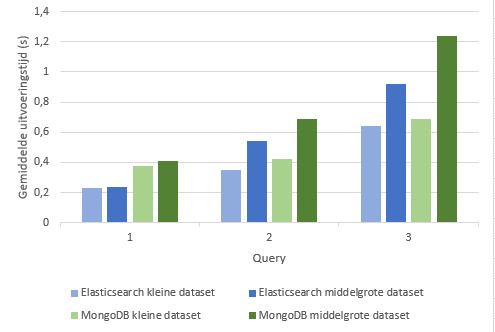
\includegraphics[width=.5\textwidth,center]{graph}
		\caption{Voorbeeld}
		\label{fig:example}
	\end{figure}
	
	
	%---------- Verwachte conclusies ----------------------------------------------
	\section{Verwachte conclusies}
	\label{sec:verwachte_conclusies}
	
	De verwachtingen voor de uitvoeringstijd bij Elasticsearch liggen hoog. Ik verwacht dat de vooral de nadelen die uit de resultaten vloeien een afschrikwekkend effect zullen hebben op veel developers maar dat de lage uitvoeringstijd veel goed kan maken. Langs de andere kant verwacht ik dat dit onderzoek aantoont dat het mogelijk is om Elasticsearch als databank te gebruiken en er dus niet altijd een koppeling met een echte databank moet zijn.
	
	%------------------------------------------------------------------------------
	% Referentielijst
	%------------------------------------------------------------------------------
	% TODO: de gerefereerde werken moeten in BibTeX-bestand ``biblio.bib''
	% voorkomen. Gebruik JabRef om je bibliografie bij te houden en vergeet niet
	% om compatibiliteit met Biber/BibLaTeX aan te zetten (File > Switch to
	% BibLaTeX mode)
	
	\phantomsection
	\printbibliography[heading=bibintoc]
	
\end{document}
